\documentclass{standalone}
\usepackage{tikz}
\usepackage{ctex,siunitx}
\setCJKmainfont{Noto Serif CJK SC}
\usepackage{tkz-euclide}
\usepackage{amsmath}
\usetikzlibrary{patterns, calc}
\usetikzlibrary {decorations.pathmorphing, decorations.pathreplacing, decorations.shapes,}
\begin{document}
\small
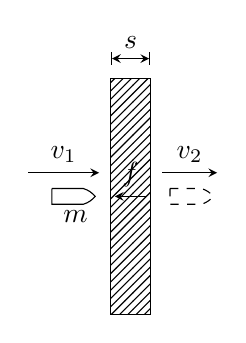
\begin{tikzpicture}[>=stealth,scale=1]
  \draw [pattern=north east lines] (-.25,-1.5) rectangle (.25, 1.5);
  \draw [|<->|] (-.25, 1.75)--node[above]{$s$} (.25,1.75);
  \draw (-1, .1) --(-.6, .1) to [bend left=15] (-.45, 0) to [bend left=15] (-.6,-.1)--(-1,-.1)--(-1,.1); 
  \node at (-.7, -.25){$m$};
  \draw [dashed] (.5, .1) --(.9, .1) to [bend left=15] (1.05, 0) to [bend left=15] (.9,-.1)--(.5,-.1)--(.5,.1); 
  \draw[->] (-1.3, .3)--node[above]{$v_1$}(-.4, .3);
  \draw[->] (.4, .3)--node[above]{$v_2$}(1.1, .3);
  \draw[->](.2,0)--node[above]{$f$}(-.2,0);
\end{tikzpicture}
\end{document}